

\tikzset{every picture/.style={line width=0.75pt}} %set default line width to 0.75pt

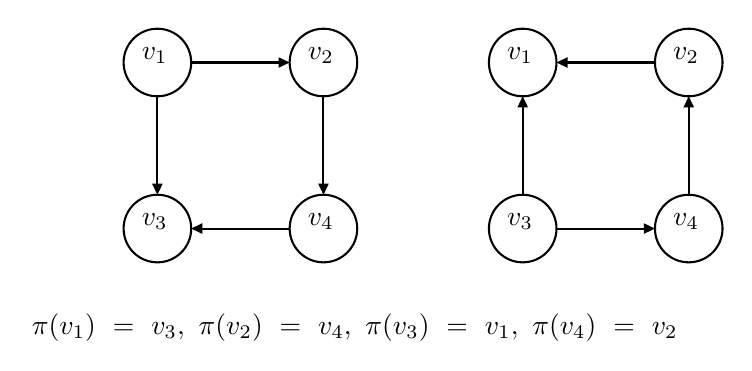
\begin{tikzpicture}[x=0.75pt,y=0.75pt,yscale=-1,xscale=1]
%uncomment if require: \path (0,194); %set diagram left start at 0, and has height of 194


% Text Node
\draw    (67, 38) circle [x radius= 16.28, y radius= 16.28]   ;
\draw (58,29.4) node [anchor=north west][inner sep=0.75pt]    {$v_{1}$};
% Text Node
\draw    (147, 118) circle [x radius= 16.28, y radius= 16.28]   ;
\draw (138,109.4) node [anchor=north west][inner sep=0.75pt]    {$v_{4}$};
% Text Node
\draw    (67, 118) circle [x radius= 16.28, y radius= 16.28]   ;
\draw (58,109.4) node [anchor=north west][inner sep=0.75pt]    {$v_{3}$};
% Text Node
\draw (5,157.4) node [anchor=north west][inner sep=0.75pt]    {$\pi ( v_{1}) \ =\ v_{3} ,\ \pi ( v_{2}) \ =\ v_{4} ,\ \pi ( v_{3}) \ =\ v_{1} ,\ \pi ( v_{4}) \ =\ v_{2}$};
% Text Node
\draw    (243, 38) circle [x radius= 16.28, y radius= 16.28]   ;
\draw (234,29.4) node [anchor=north west][inner sep=0.75pt]    {$v_{1}$};
% Text Node
\draw    (323, 38) circle [x radius= 16.28, y radius= 16.28]   ;
\draw (314,29.4) node [anchor=north west][inner sep=0.75pt]    {$v_{2}$};
% Text Node
\draw    (323, 118) circle [x radius= 16.28, y radius= 16.28]   ;
\draw (314,109.4) node [anchor=north west][inner sep=0.75pt]    {$v_{4}$};
% Text Node
\draw    (243, 118) circle [x radius= 16.28, y radius= 16.28]   ;
\draw (234,109.4) node [anchor=north west][inner sep=0.75pt]    {$v_{3}$};
% Text Node
\draw    (147, 38) circle [x radius= 16.28, y radius= 16.28]   ;
\draw (138,29.4) node [anchor=north west][inner sep=0.75pt]    {$v_{2}$};
% Connection
\draw    (67,54.28) -- (67,98.72) ;
\draw [shift={(67,101.72)}, rotate = 270] [fill={rgb, 255:red, 0; green, 0; blue, 0 }  ][line width=0.08]  [draw opacity=0] (5.36,-2.57) -- (0,0) -- (5.36,2.57) -- cycle    ;
% Connection
\draw    (130.72,118) -- (86.28,118) ;
\draw [shift={(83.28,118)}, rotate = 360] [fill={rgb, 255:red, 0; green, 0; blue, 0 }  ][line width=0.08]  [draw opacity=0] (5.36,-2.57) -- (0,0) -- (5.36,2.57) -- cycle    ;
% Connection
\draw    (147,54.28) -- (147,98.72) ;
\draw [shift={(147,101.72)}, rotate = 270] [fill={rgb, 255:red, 0; green, 0; blue, 0 }  ][line width=0.08]  [draw opacity=0] (5.36,-2.57) -- (0,0) -- (5.36,2.57) -- cycle    ;
% Connection
\draw    (83.28,38) -- (127.72,38) ;
\draw [shift={(130.72,38)}, rotate = 180] [fill={rgb, 255:red, 0; green, 0; blue, 0 }  ][line width=0.08]  [draw opacity=0] (5.36,-2.57) -- (0,0) -- (5.36,2.57) -- cycle    ;
% Connection
\draw    (306.72,38) -- (262.28,38) ;
\draw [shift={(259.28,38)}, rotate = 360] [fill={rgb, 255:red, 0; green, 0; blue, 0 }  ][line width=0.08]  [draw opacity=0] (5.36,-2.57) -- (0,0) -- (5.36,2.57) -- cycle    ;
% Connection
\draw    (243,101.72) -- (243,57.28) ;
\draw [shift={(243,54.28)}, rotate = 450] [fill={rgb, 255:red, 0; green, 0; blue, 0 }  ][line width=0.08]  [draw opacity=0] (5.36,-2.57) -- (0,0) -- (5.36,2.57) -- cycle    ;
% Connection
\draw    (259.28,118) -- (303.72,118) ;
\draw [shift={(306.72,118)}, rotate = 180] [fill={rgb, 255:red, 0; green, 0; blue, 0 }  ][line width=0.08]  [draw opacity=0] (5.36,-2.57) -- (0,0) -- (5.36,2.57) -- cycle    ;
% Connection
\draw    (323,101.72) -- (323,57.28) ;
\draw [shift={(323,54.28)}, rotate = 450] [fill={rgb, 255:red, 0; green, 0; blue, 0 }  ][line width=0.08]  [draw opacity=0] (5.36,-2.57) -- (0,0) -- (5.36,2.57) -- cycle    ;

\end{tikzpicture}